
\begin{figure}[h!]
    \centering
    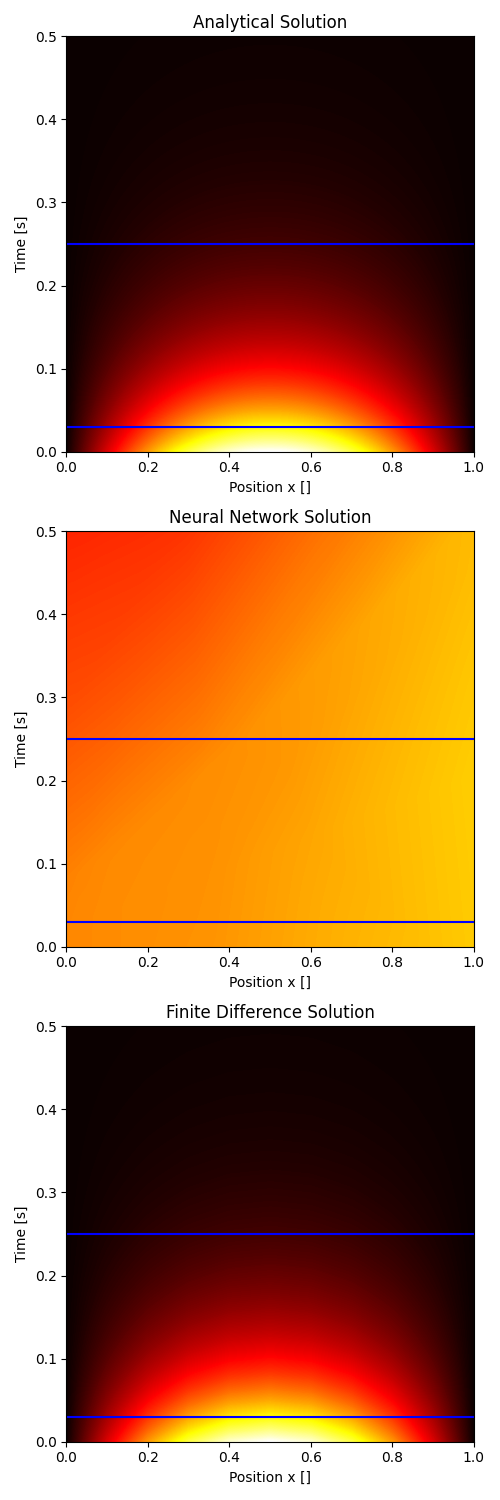
\includegraphics[width=1.0\linewidth]{project_3/plots/heat_map_comparison.pdf}
    \caption{The analytical solution to the heat equation as well as the result from the finite difference method and the neural network model. A common colorbar is displayed. }
    \label{fig:heatmaps}
\end{figure}

The results from the finite difference method and the NN are presented in Fig. \ref{fig:heatmaps}.
Compared to the analytical solution, the output of the neural network model has a MSE of $ 3.41 \times 10^{-5}$ while the finite difference method yields a MSE of $2.52 \times 10^{-7}$
Looking at the respective methods output in Fig. \ref{fig:heatmaps}, their is no noticeable difference by eye between any of the three.  
This is well reflected in the very low MSE-value for both methods. 

\begin{figure}[h!]
    \centering
    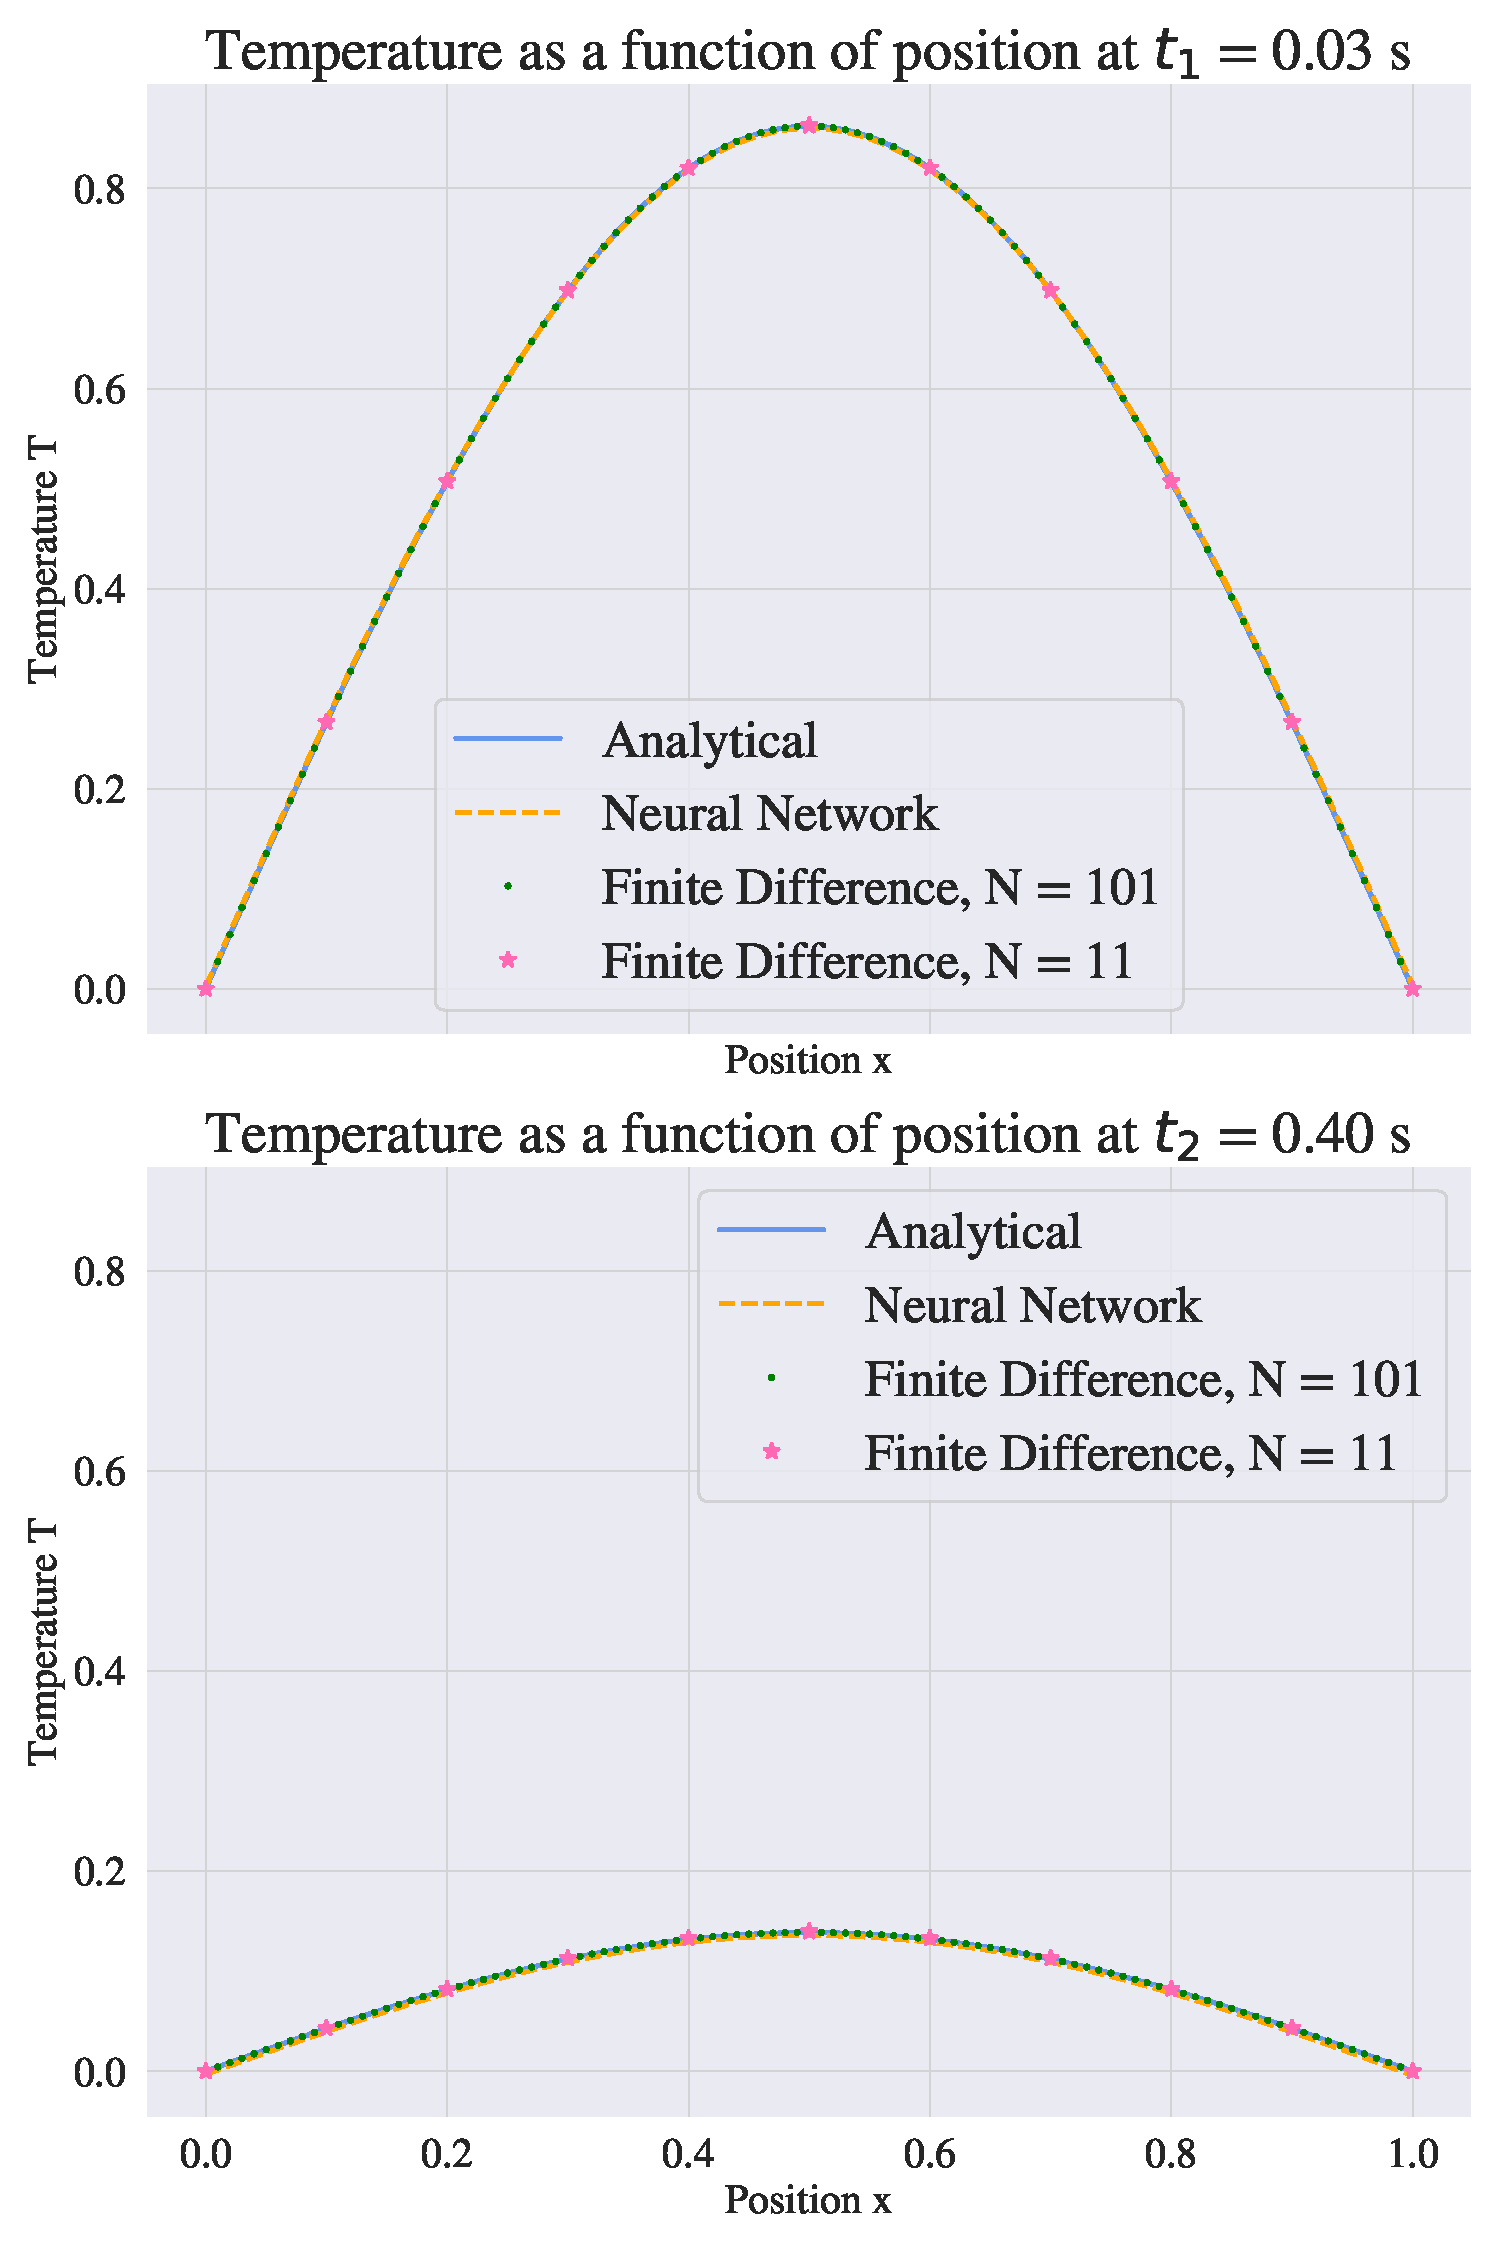
\includegraphics[width=1.0\linewidth]{project_3/plots/time_slices_comparison.pdf}
    \caption{The temperate for specific times for the analytical solution, as well as the output from the finite difference method and the neural network predictions. The discretization along the x-axis is different for each method. The analytical one is plotted with 1000 points, the finite difference method with 10 points and the neural network predictions with 100. }
    \label{fig:timeslices}
\end{figure}



\begin{figure}[h!]
    \centering
    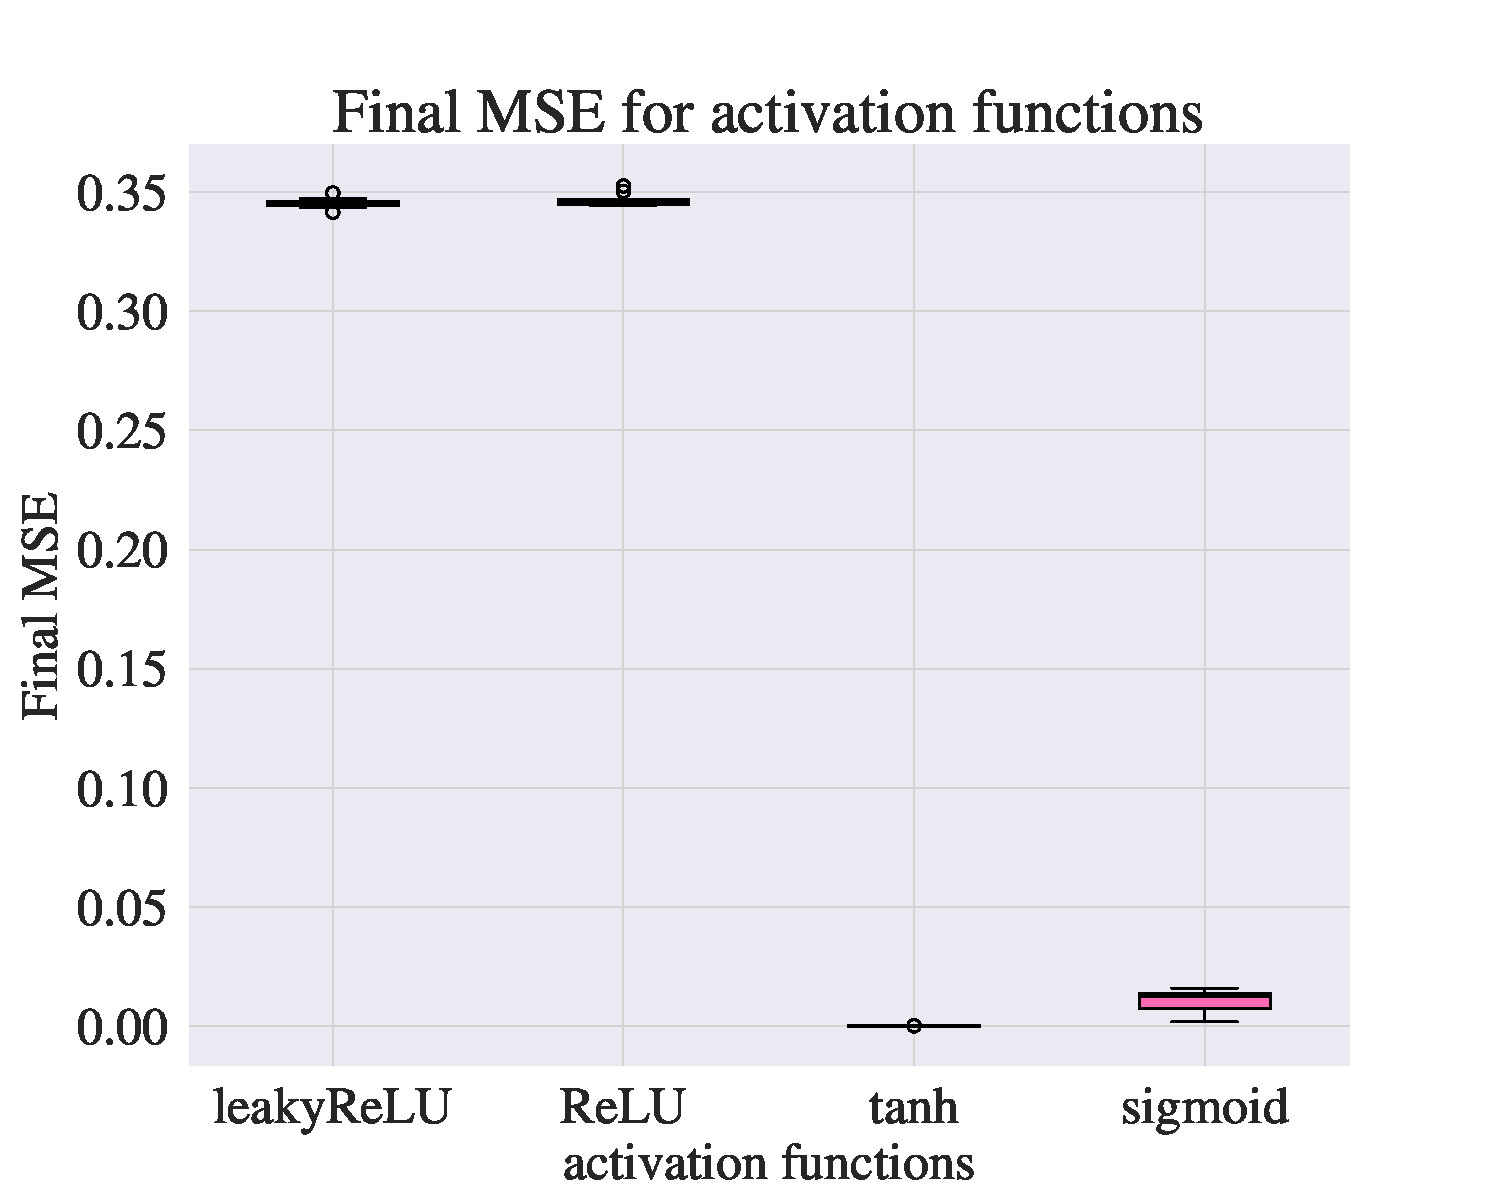
\includegraphics[width=1.0\linewidth]{project_3/plots/activation_search.pdf}
    \caption{Boxplots showcasing the final MSE value compared to the analytical solution for different activation functions. Each model is ran 10 times.}
    \label{fig:boxplots_activations}
\end{figure}

\begin{figure}[h!]
    \centering
    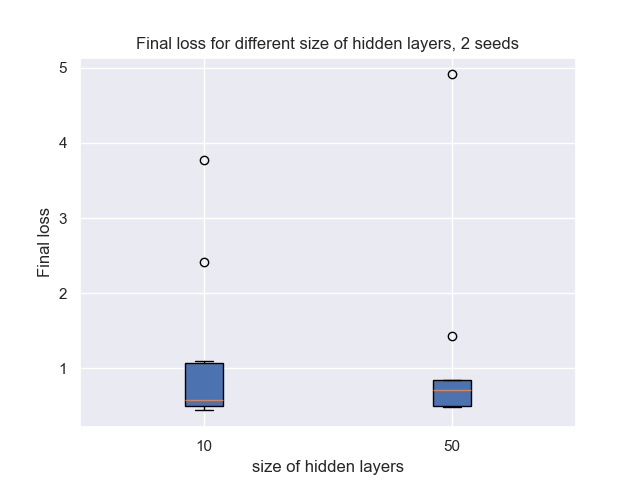
\includegraphics[width=1.0\linewidth]{project_3/plots/value_layers_search.png}
    \caption{Boxplots showcasing the final MSE value compared to the analytical solution for different sizes for the hidden layers. Each model is ran 10 times. \mia{this is wrong plot for now}}
    \label{fig:boxplots_size_of_layers}
\end{figure}

\begin{figure}[h!]
    \centering
    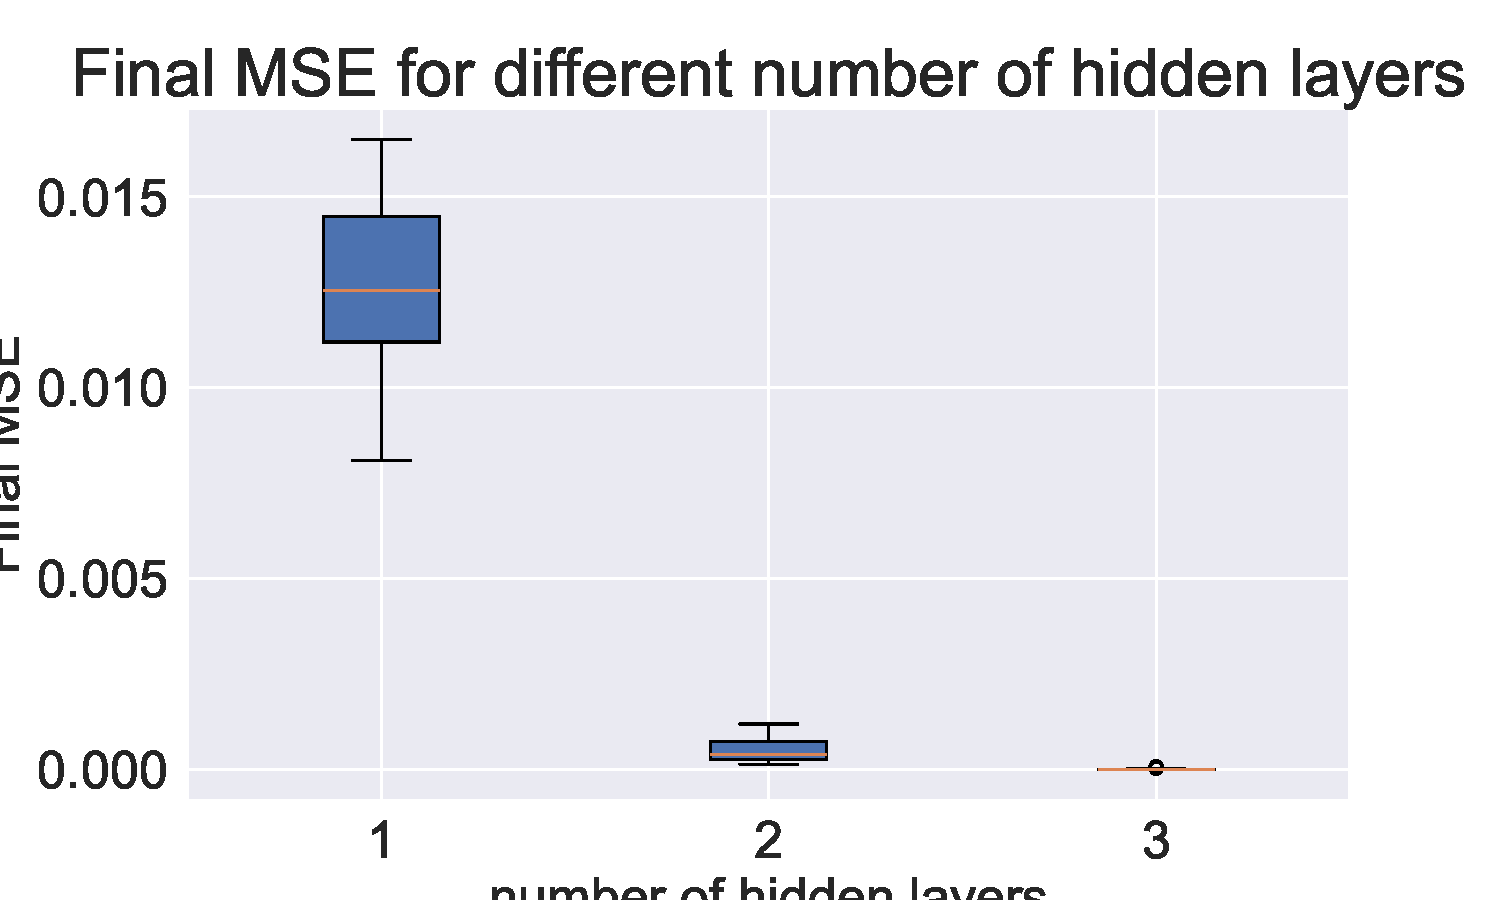
\includegraphics[width=1.0\linewidth]{project_3/plots/n_layers_search.pdf}
    \caption{Boxplots showcasing the final MSE value compared to the analytical solution for different number of hidden layers. Each model is ran 10 times.}
    \label{fig:boxplots_number_of_hidden_layers}
\end{figure}

